\documentclass[a4paper,11pt]{article}

\newcommand{\authorinfo}{Paul Bienkowski, Konstantin Kobs}
\newcommand{\titleinfo}{Robotics Assignment \#05}

% PREAMBLE ===============================================================

\usepackage[german,ngerman]{babel}
\usepackage[utf8]{inputenc}
\usepackage[T1]{fontenc}
\usepackage[top=1.3in, bottom=1in, left=1.0in, right=0.6in]{geometry}
\usepackage{lmodern}
\usepackage{amssymb}
\usepackage{mathtools}
\usepackage{amsmath}
\usepackage{enumerate}
\usepackage{pgfplots}
\usepackage{breqn}
\usepackage{tikz}
\usepackage{fancyhdr}
\usepackage{multicol}
\usepackage{gensymb}
\usepackage{listings}
\lstset{tabsize=2}

\allowdisplaybreaks

\usetikzlibrary{calc}
\usetikzlibrary{patterns}

\author{\authorinfo}
\title{\titleinfo}
\date{\today}

\pagestyle{fancy}
\fancyhf{}
\fancyhead[L]{\authorinfo}
\fancyhead[R]{\titleinfo}
\fancyfoot[C]{\thepage}

\begin{document}
\maketitle
\begin {enumerate}
	\item[\textbf{Task 5.1.}]
		We wrote a script in Python to calculate the basis splines. These are the plots we got from our code:<
		
		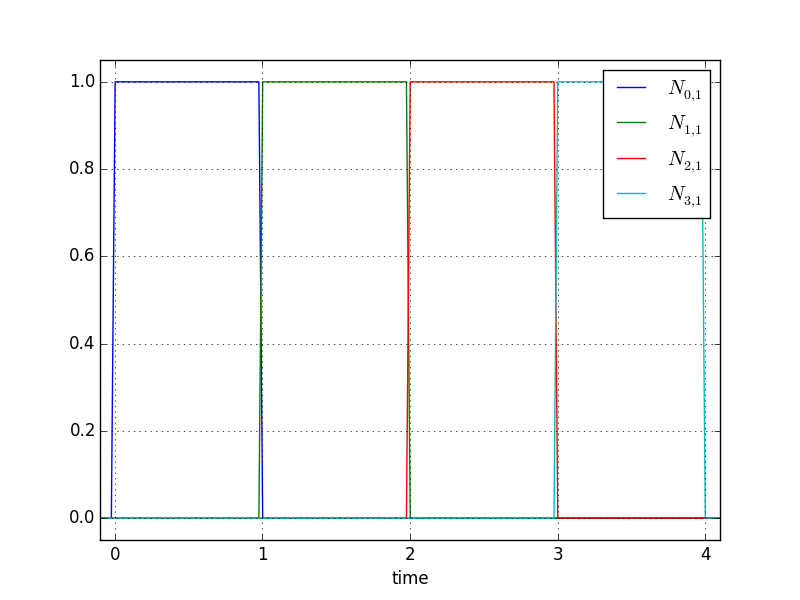
\includegraphics[width=0.5\textwidth]{5-1-k=1}
		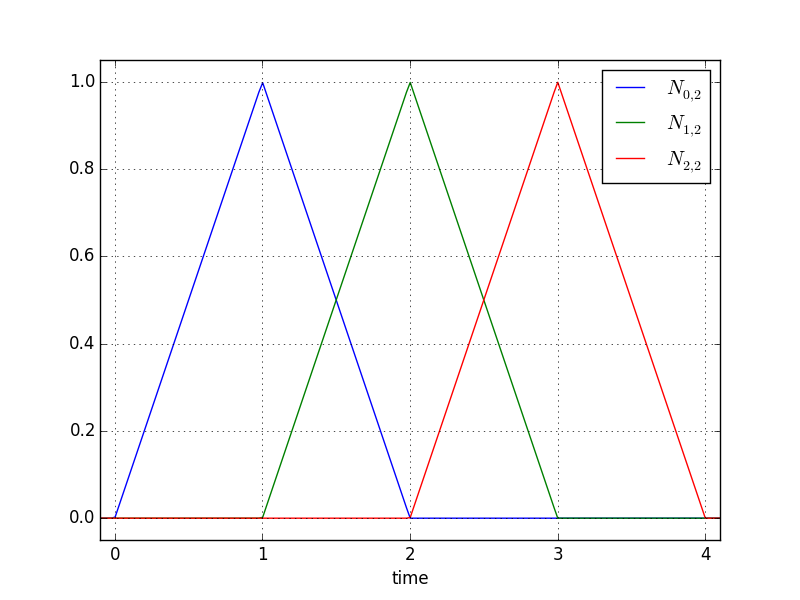
\includegraphics[width=0.5\textwidth]{5-1-k=2}
		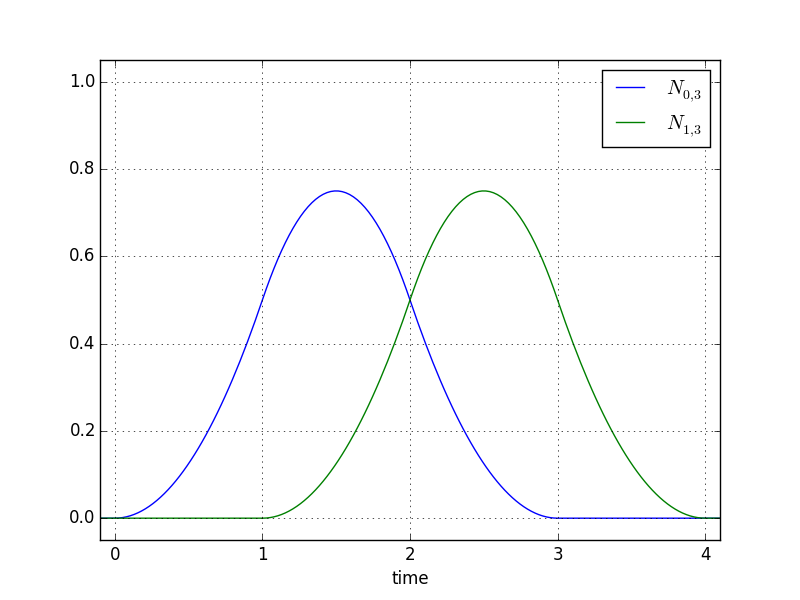
\includegraphics[width=0.5\textwidth]{5-1-k=3}
		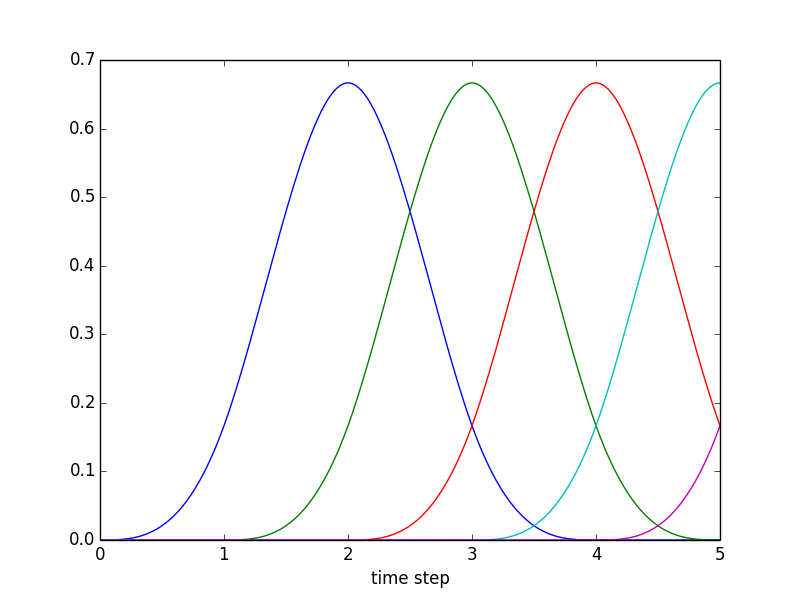
\includegraphics[width=0.5\textwidth]{5-1-k=4}
		
		We wrote the following code:
		
		\lstinputlisting[language=python, frame=single, breaklines=true]{5.1.py}
		
	\item[\textbf{Task 5.2.}]
		For $k = 1$, we can just use the given formula on slide 220:
		$$N_{i,1}(t) = \begin{cases}
			1 & \text{for } t_{i} \leq t < t_{i+1}\\
			0 & \text{else}
		\end{cases}$$
		
		For $k = 2$, we need to insert this definition into the recursive definition
		$$N_{i,k}(t) = \frac{t-t_i}{t_{i+k-1}-t_i} N_{i, k-1}(t) + \frac{t_{i+k}-t}{t_{i+k}-t_{i+1}} N_{i+1, k-1}(t)$$
		Since $t$ can't be satisfying both summands, we can split this up into the desired direct definition. Therefore, for $k = 2$:
		$$N_{i,2}(t) = \begin{cases}
			\frac{t-t_i}{t_{i+k-1}-t_i} & \text{for } t_{i} \leq t < t_{i+1}\\
			\frac{t_{i+k}-t}{t_{i+k}-t_{i+1}} & \text{for } t_{i+1} \leq t < t_{i+2}\\
			0 & \text{else}
		\end{cases}$$
		For the last case, we need to input this definition again into the recursive definition and think about, what values $t$ can have. Then we can define:
		$$N_{i,3}(t) = \begin{cases}
			\left( \frac{t-t_i}{t_{i+k-1}-t_i} \right)^2 & \text{for } t_{i} \leq t < t_{i+1}\\
			\frac{t-t_i}{t_{i+k-1}-t_i} \cdot \frac{t_{i+k}-t}{t_{i+k}-t_{i+1}} + \frac{t_{i+k}-t}{t_{i+k}-t_{i+1}} \cdot \frac{t-t_{i+1}}{t_{i+k}-t_{i+1}} & \text{for } t_{i+1} \leq t < t_{i+2}\\
			\frac{t_{i+k}-t}{t_{i+k}-t_{i+1}} \cdot \frac{t_{i+k+1}-t}{t_{i+k+1}-t_{i+2}} & \text{for } t_{i+2} \leq t < t_{i+3}\\
			0 & \text{else}
		\end{cases}$$
		
		It is important to see, that whenever the second case of the $k = 2$ definition is inserted, $i$ has to be increased by one, because it is passed so to the definition.
		
	\item[\textbf{Task 5.3.}]
		\begin{align*}
			L_0(x) &= \frac{(x-1)(x-3)(x-5)}{(0-1)(0-3)(0-5)}\\
					&= \frac{(x^2 - 4x + 3)(x-5)}{-15}\\
					&= \frac{x^3 - 9x^2 + 23x -15}{-15}\\
					&= - \frac{1}{15} x^3 + \frac{9}{15} x^2 - \frac{23}{15} x + 1\\
			L_1(x) &= \frac{(x-0)(x-3)(x-5)}{(1-0)(1-3)(1-5)}\\
					&= \frac{x^3 - 8x^2 + 15x}{8}\\
					&= \frac{1}{8} x^3 - x^2 + \frac{15}{8} x\\
			L_2(x) &= \frac{(x-0)(x-1)(x-5)}{(3-0)(3-1)(3-5)}\\
					&= \frac{x^3 - 6x^2 + 5x}{-12}\\
					&= -\frac{1}{12} x^3 + \frac{1}{2} x^2 - \frac{5}{12} x\\
			L_3(x) &= \frac{(x-0)(x-1)(x-3)}{(5-0)(5-1)(5-3)}\\
					&= \frac{x^3 - 4x^2 + 3x}{40}\\
					&= \frac{1}{40} x^3 - \frac{1}{10} x^2 + \frac{3}{40} x\\
			p_I(x) &= y_0 L_0(x) + y_1 L_1(x) + y_2 L_2(x) + y_3 L_3(x)\\
					&= 1 \cdot L_0(x) + 3 \cdot L_1(x) - 2 \cdot L_2(x) + 4 \cdot L_3(x)\\
					&= \left(- \frac{1}{15} x^3 + \frac{9}{15} x^2 - \frac{23}{15} x + 1 \right) + 3 \cdot \left(\frac{1}{8} x^3 - x^2 + \frac{15}{8} x\right)\\
					&\qquad - 2 \cdot \left(-\frac{1}{12} x^3 + \frac{1}{2} x^2 - \frac{5}{12} x \right) + 4 \cdot \left(\frac{1}{40} x^3 - \frac{1}{10} x^2 + \frac{3}{40} x \right)\\
					&= - \frac{1}{15} x^3 + \frac{9}{15} x^2 - \frac{23}{15} x + 1 + \frac{3}{8} x^3 - 3x^2 + \frac{45}{8} x\\
					&\qquad + \frac{1}{6} x^3 - x^2 + \frac{5}{6} x + \frac{1}{10} x^3 - \frac{2}{5} x^2 + \frac{3}{10} x\\
					&= \left( -\frac{1}{15} + \frac{3}{8} + \frac{1}{6} + \frac{1}{10} \right) x^3 + \left( \frac{9}{15} - 3 - 1 - \frac{2}{5} \right) x^2 + \left( -\frac{23}{15} + \frac{45}{8} + \frac{5}{6} + \frac{3}{10} \right) x + 1 \\
					&= \frac{69}{120} x^3 -\frac{19}{5} x^2 + \frac{627}{120} x + 1 \\
					&= \frac{23}{40} x^3 -\frac{19}{5} x^2 + \frac{209}{40} x + 1\\
		\end{align*}
	
		We then used Python to visualize the data. This is what we've got:
		
		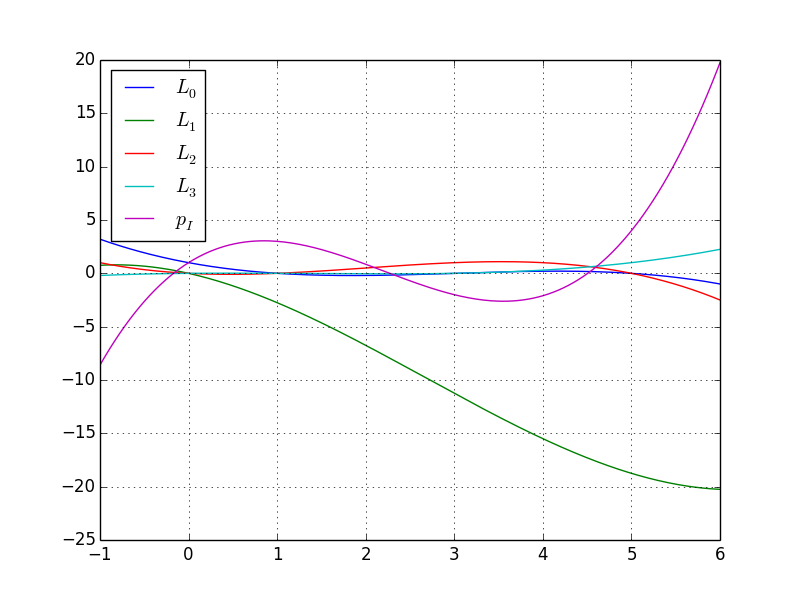
\includegraphics[width=\textwidth]{5-3}
		
		This is the code we used:
		
		\lstinputlisting[language=python, frame=single, breaklines=true]{5.3.py}
		
	\item[\textbf{Task 5.4.}]
		
		
		
\end {enumerate}
\end{document}
